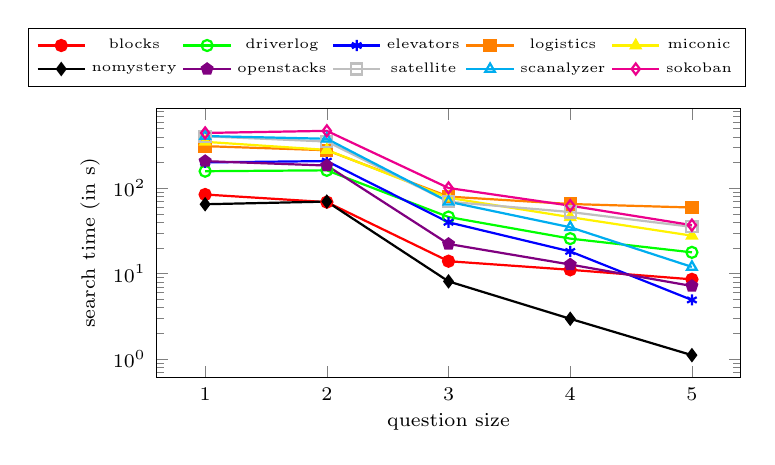
\begin{tikzpicture}[scale=1]
\tiny
    \begin{axis}[
    width = 9cm,
    height=5cm,
    enlarge x limits = 0.1,
    enlarge y limits = 0.1,
    ymode=log,
    xmin = 1,
	xmax = 5,
	xtick={1,2,3,4,5},
	xlabel = {question size},
	x label style = {font=\scriptsize},
	ylabel = {search time (in s)},
	legend style={at={(1.01,1.30)}},
	y label style = {font=\scriptsize},
	legend columns=5,
	x tick label style = {font=\scriptsize, yshift=-0.05cm},
	y tick label style = {font=\scriptsize, xshift=-0.05cm},
]
\addplot[thick, red, mark=*,
]
	plot coordinates {
		(1, 84.53)
		(2, 68.87)
		(3, 13.99)
		(4, 11.1)
		(5, 8.58)
	};
\addlegendentry{blocks}
\addplot[thick, green, mark=o,
]
	plot coordinates {
		(1, 158.49)
		(2, 162.32)
		(3, 46.09)
		(4, 25.74)
		(5, 17.77)
	};
\addlegendentry{driverlog}
\addplot[thick, blue, mark=asterisk,
]
	plot coordinates {
		(1, 201.02)
		(2, 208.31)
		(3, 39.96)
		(4, 18.21)
		(5, 4.92)
	};
\addlegendentry{elevators}
\addplot[thick, orange, mark=square*,
]
	plot coordinates {
		(1, 311.58)
		(2, 279.05)
		(3, 79.89)
		(4, 65.44)
		(5, 59.51)
	};
\addlegendentry{logistics}
\addplot[thick, yellow, mark=triangle*,
]
	plot coordinates {
		(1, 350.17)
		(2, 281.58)
		(3, 77.4)
		(4, 45.93)
		(5, 27.85)
	};
\addlegendentry{miconic}
\addplot[thick, black, mark=diamond*,
]
	plot coordinates {
		(1, 65.03)
		(2, 69.83)
		(3, 8.12)
		(4, 2.96)
		(5, 1.11)
	};
\addlegendentry{nomystery}
\addplot[thick, violet, mark=pentagon*,
]
	plot coordinates {
		(1, 208.06)
		(2, 184.65)
		(3, 22.27)
		(4, 12.79)
		(5, 7.17)
	};
\addlegendentry{openstacks}
\addplot[thick, lightgray, mark=square,
]
	plot coordinates {
		(1, 406.77)
		(2, 352.83)
		(3, 69.58)
		(4, 52.73)
		(5, 35.34)
	};
\addlegendentry{satellite}
\addplot[thick, cyan, mark=triangle,
]
	plot coordinates {
		(1, 409.17)
		(2, 380.07)
		(3, 69.56)
		(4, 34.95)
		(5, 12.0)
	};
\addlegendentry{scanalyzer}
\addplot[thick, magenta, mark=diamond,
]
	plot coordinates {
		(1, 444.74)
		(2, 470.68)
		(3, 100.78)
		(4, 62.61)
		(5, 37.0)
	};
\addlegendentry{sokoban}

    \end{axis}

\end{tikzpicture}
\\
